\def\year{2018}\relax
%File: formatting-instruction.tex
\documentclass[letterpaper]{article} %DO NOT CHANGE THIS
\usepackage{aaai18}  %Required
\usepackage{times}  %Required
\usepackage{helvet}  %Required
\usepackage{courier}  %Required
\usepackage{url}  %Required
\usepackage{graphicx}  %Required
\usepackage{caption}
\usepackage{amsmath}
\frenchspacing  %Required
\setlength{\pdfpagewidth}{8.5in}  %Required
\setlength{\pdfpageheight}{11in}  %Required
%PDF Info Is Required:
  \pdfinfo{
/Title (Model Comparison in Sentiment Analysis Domain Based on Amazon Reviews)
/Author (Linhai Zhang; Lixia Yi; Hanmo Li; Xinjie Ye; Shiwei Cao)}
\setcounter{secnumdepth}{0}  
 \begin{document}
% The file aaai.sty is the style file for AAAI Press 
% proceedings, working notes, and technical reports.
%
\title{Model Comparison in Sentiment Analysis Domain Based on Amazon Reviews}
\author{Linhai Zhang; Lixia Yi; Hanmo Li; Xinjie Ye; Shiwei Cao\\
University of Wisconsin-Madison\\
702 West Johnson Street Suite 1101\\
Madison, Wisconsin 53715-1007\\
}
\maketitle
\begin{abstract}
This project tends to compare multiple models in sentiment analysis domain based on Amazon reviews. We run the experiment for LogisticRegression, NaiveBayes, SVM, NBSVM, XGBoost and LSTM on same kind of dataset to compare running time, memory usage and accuracy. As a result.....

\end{abstract}
\section{Introduction}
\subsection{Background}
importance of sentiment, existing method, compare to find, 
Nowadays, what people think is of great concern. Fortunately, with the growth of available opinion-rich resources, such as online review and blogs, and along with new technologies, such as machine learning and sentiment analysis, we are able to extract information from these resources and understand the opinions of others. However, it's not a easy task, as we have to teach machines to do what human brains do to understand others' comments.

This project tends to compare multiple popular models used in sentiment analysis based on Amazon reviews. We will compare the running time, memory usage and accuracy of each model to find out when, where and which model fits best. 

\subsection{Data Introduction}
We get our data from Dr. Julian McAuley's \ref{he2016ups} Amazon dataset. The dataset contains product reviews and metadata from Amazon, including 142.8 million reviews spanning May 1996 - July 2014.The dataset includes reviews (ratings, text, helpfulness votes), product metadata (descriptions, category information, price, brand, and image features), and links (also viewed/also bought graphs). \par
For our project, we choose the data only for electronics, which contains 1689188 reviews. Since our project focus on text classification. We only keep the review texts and ratings in the data. Table 1 is an example of the data.\par
\begin{table}[htb]
\caption{Example of Amazon Review Data} % title of Table
\resizebox{\columnwidth}{!}{
\begin{tabular}{|p{1cm}|p{1cm}|p{6cm}|} % centered columns (4 columns)
\hline %inserts double horizontal lines
Index & Rating & Review \\ [0.5ex] % inserts table
%heading
\hline % inserts single horizontal line
1 & 5 & I bought this for my husband who plays the piano. He is having a wonderful time playing these old hymns... \\ [1ex] % [1ex] adds vertical space
\hline %inserts single line
\end{tabular}
}
\end{table}

\subsection{Experiment Design}

First, we clean the data set and extract the train and test set from cleaned data. Then each model will use same train and test set, measure the running time and memory usage of model and use the same criterion to calculate the accuracy. Finally we will do comparison between all the models and summarize the findings.

\section{Model Description}

\subsection{Logistic Regression}

multinomial logistic regression(LR) is a classification method that generalizes logistic regression to multiclass problems, i.e. with more than two possible discrete outcomes. That is, it is a model that is used to predict the probabilities of the different possible outcomes of a categorically distributed dependent variable, given a set of independent variables (which may be real-valued, binary-valued, categorical-valued, etc.).

Multinomial logistic regression is known by a variety of other names, including polytomous LR, multiclass LR, softmax regression, multinomial logit, maximum entropy (MaxEnt) classifier, conditional maximum entropy model.

\subsection{Naive Bayes}

Naive Bayes is a baseline algorithm to tackle the text classification and sentiment analysis problem. Its simplexity and robust makes it popular in the text processing domain. The critical function in Naive bayes is as follows: \cite{pedregosa2011scikit}
$$p(y|x_1,...,x_n) = \frac{p(y)\prod_i p(x_i|y)}{p(x_1,...,x_n)}$$
Problem here is to figure out the value of $p(x_i|y)$ from samples. There are two common ways to do this.
\subsubsection{Gaussian Naive Bayes}

Under the Gaussian assumption, the $p(x_i|y)$ can be calculated as the equation follows.

$$p(x_i|y) = \frac{1}{\sqrt{2\pi \sigma_y^2}}exp(-\frac{(x_i-\mu_y)^2}{2\sigma_y^2})$$

The parameters $\sigma_y$ and $\mu_y$ are estimated by the maximum likehood method.

\subsubsection{Multinomial Naive Bayes}

This method is what we have learnt from class. That is, the $p(x_i|y)$ is calculated using the following equation.

$$p(x_i|y)=\frac{N_{yi}+\alpha}{N_y+\alpha n}$$

$\alpha$ here is the smooth parameter.

\subsection{SVM}

SVM is another baseline algorithm for the sentiment analysis tasks. The tricky part for SVM is to choose a proper kernal. Here we tried several popular kernals and compared their model performances(shown in the following table).

\subsection{NBSVM}

NB-SVM is a powerful algorithm introduced by Sida Wang and Christopher D. Manning(2012)\cite{wang2012baselines}, which is designed to tackle the sentiment and topic classification tasks. It's now one of the most popular algorithms used in Kaggle community for the text calssification competitions.

The intuitive insight for NB-SVM is that NB beats the SVM for short snippet sentiment task while SVM performs better for longer documents. Thus by combining these two baseline algorithms together, NB-SVM inherits both advantages for NB and SVM and outperforms most published algorithm in the sentiment analysis domain.

The process for NB-SVM is to firstly extract the NB features, then use them to fit the SVM model. The SVM model here can be replaced by other calssification methods, like logistic regression model etc..

The technical details about this algorithm is shown as follows\cite{lebret2014n}(binary classification problem with $y=(1,-1)$).

Suppose $D = (d_1,d_2,...,d_n)$ is a set of text documents and each text documents $d_i$ contains a set of n-grams. We denote ngm = $(ngm_1,ngm_2,..,ngm_N)$ as the set of count vectors for all n-grams extracted from $D$. $ngm^i_t$ represents the number of occurence of $t$th n-gram in document i. Defining $p = 1+\sum_{i:y_i=1}ngm^i$ and $q=1+\sum_{i:y_i=-1}ngm^i$. To determine how important n-grams are for the classes y, defining the log ratio $r$:

$$r=log(\frac{p/||p||_1}{q/||q||_1})$$

Then to get better performance, we need to binarize ngm. That is, set ngm as $\hat{ngm}^{i}=1(ngm^i>0)$. To get the NB feature, we only need to product $\hat{r}$ and $\hat{ngm}$ together. Finally, by using the NB features as the input for SVM, we can get the final result of NB-SVM algorithm.

\subsection{Xgboost}

Aiming to provide a "Scalable, Portable and Distributed Gradient Boosting (GBM, GBRT, GBDT) Library", XGBoost is an famous open source library which provides the gradient boosting framework. Generally speaking, it combines several prediction results from different decision trees, which is so called 'ensemable of weak prediction model'. The algorithm initially introduced by Tianqi Chen in 2016 and soon became popular among Kaggle community.(Wiki Xgboost)\par
When using single algorithms to conduct the cross validation, the preformance of XGBoost had been among the top tier. Therefore XGBoost was one of the top candidates in the following model combination step. In fact, when we chose NBSVM as the first model, Xgboost performed best as the second model comparing with other machine learning algorithms.

\subsection{LSTM}

In this part, we will explore how deep neural network model with a long short time memory(LSTM) layer works for our data. 
Firstly, we learn the architecture of the model. It is very hard to learn the structure of the model, especially for deep learning model. So, in this project, we just use the simplest structure: one word embedding layer, one LSTM layer and one full connection layer to output the prediction. 
Parameter tuning part could be very crucial to this method. But we do not have enough time to do parameter tuning for all sample sizes. So, we only do parameter tuning for size = 100000 and use this setup for all sizes. This may affect the accuracy of our models. \par

For our LSTM model. We care about four parameters most. They are:
\begin{itemize}
\item Number of kernels in word embedding layer;
\item Number of kernels in LSTM layer;
\item Dropout rate;
\item Number of epochs;
\end{itemize}
We did four experiments for the four parameters. Here is the setup for the experiments.
\begin{itemize}
\item Train on 10000 data;
\item Test on 5000 data;
\item Record the RMSE of train data and test data;
\end{itemize}

\begin{center}
  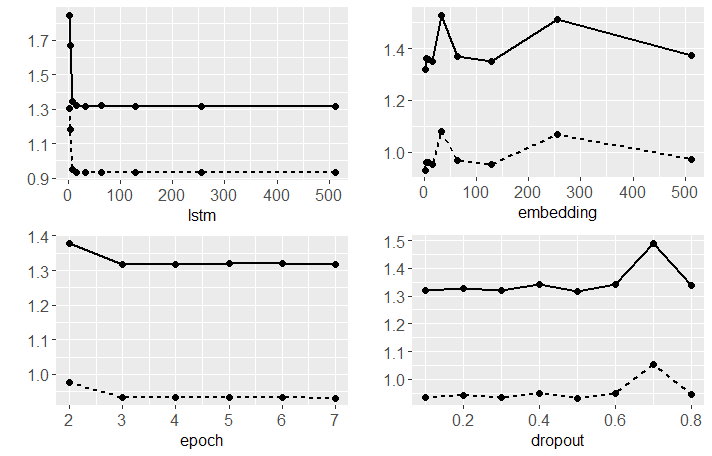
\includegraphics[width=\columnwidth]{../Plots/lstm_parameters.png}
  \captionof{figure}{Parameter tuning for LSTM model,dash line for RMSE of train set, solid line for test set}
\end{center}

Based on Figure.1, here is our final model setup:
\begin{itemize}
\item Dropout rate: 0.2
\item Number of epochs: 4
\item Number of kernels in embedding: 128
\item Number of kernels in LSTM network: 128
\end{itemize}
For the activation function and loss function, we look up for literature and use sigmoid function for activation function and mean square root function for loss function.
By now we have our model ready. We will use this model to do evaluation in the next part.

\section{Data Engineering}
\subsection{Data cleaning}
Before we start fitting the model, some data cleaning processes are necessary. Because, if we do not clean the raw texts and use them directly, the dimension of the feature matrix will be ultra-high, which will not only slow down the modeling fitting, but also reduces the accuracy. 
Our data cleaning processes contain the following step:
\begin{itemize}
\item Remove punctuations except ! and ?;
\item Transfer into lower case;
\item Remove stopwords;
\item Normalize the verbs and nouns;
\end{itemize}
In the first step, we keep "!" and "!" because these two punctuations contain strong emotions. In the second step, there may be some all-capital words in the reviews to show the reviews? angry or surprise. But it is hard to recognize, so we ignore them, which may cause a very small loss in accuracy. In the third step, a stopwords list is basically a collection of most common used words. But here we edited this list to keep the words such as "never" that we think contain strong emotions. In the fourth step, we do this because we want to make our feature matrix smaller.
\subsection{Feature Matrix}
In this part, we will transfer the cleaned review texts into different kinds of feature matrix that could be put into all kinds of models. In this project, we will mainly use two kinds of methods to do this step. \par
The first one is TF/IDF method. TF/IDF method basically gives one score for every word to vectorize the texts. In detail, we remove all words with occurrences under 3 in the whole text as well as frequency above 0.9 in the whole text. These two thresholds are learned from our previous project on text classification. What?s more, we consider both single words and the combination of two words.\par
The second one is bag-of-word method. In this method, we just keep top 50000 frequent words and count their occurrence in every review. Again, the threshold 50000 is choose from the previous experience. Here are examples to show how final feature matrixes look like.


\begin{table}[htb]
\caption{Example of TF/IDF Feature Matrix} % title of Table
\resizebox{\columnwidth}{!}{
\begin{tabular}{ccccc} % centered columns (4 columns)
\hline %inserts double horizontal lines
Index & $\text{Word}_1$ & $\text{Word}_2$ & ... & $\text{Word}_{50000}$ \\ [0.5ex] % inserts table
%heading
\hline % inserts single horizontal line
1 & 0.2312 & 0.1983 & ... & 0.7823 \\ [1ex] % [1ex] adds vertical space
2 & 0.6547 & 0.0023 & ... & 0.8731 \\
...\\
1689188 & 0.1231 & 0.6542 & ... & 0.0025\\
\hline %inserts single line
\end{tabular}
}
\end{table}

\begin{table}[htb]
\caption{Example of Bag-of-word Feature Matrix} % title of Table
\resizebox{\columnwidth}{!}{
\begin{tabular}{ccccc} % centered columns (4 columns)
\hline %inserts double horizontal lines
Index & $\text{Word}_1$ & $\text{Word}_2$ & ... & $\text{Word}_{50000}$ \\ [0.5ex] % inserts table
%heading
\hline % inserts single horizontal line
1 & 1 & 0 & ... & 2 \\ [1ex] % [1ex] adds vertical space
2 & 0 & 1 & ... & 0 \\
...\\
1689188 & 0 & 0 & ... & 1\\
\hline %inserts single line
\end{tabular}
}
\end{table}

\section{Model Evaluation}
We compared the methods described in the last section in regard of time, prediction accuracy and memory usage. Several interesting issues revealed themselves during the evaluation which will be discussed in the upcoming part of this section. It is noticeable that not every method had been run multiple times, such as Xgboost and LSTM, due to their exhaustive runtime. Furthermore, we excluded the a thorough evaluation of SVM in this section since the results of SVM on small datasets were performing far worse than the other methods in regard of accuracy and runtime. This is an interesting contradiction to our prior believe suggested by \cite{rennie2001improving} and \cite{pang2002thumbs} and we believe that a more careful study on this phenomenon should be introduced.8

% Subsection
% There is still a problem with \ref{}
\subsection{Execution time and Prediction Accuracy}
There is a trade off between accuracy and speed as shown in Figure \ref{fig:runtime} and Figure \ref{fig:mse}. However, this conclusion doesn't hold rigidly since we excluded SVM in our evaluation. We've run SVM on a train size of 50,000 and after running it about 5 hours, the MSE of the prediction were about 2.0082, which means that SVM took 300 times longer than the NB or NBSVM yet yielding a far worse MSE than the two methods under the same training size. Although we believe that the prediction performance of SVM will increase if a larger training set is used, we couldn't convince ourself that it could exceed the accuracy of either NB or NBSVM within a reasonable time. In general, we could observe that computational more demanding algorithms do better in prediction.

It was out of our expectation that both NB and SVM, which we believed would do better in text classification, performed particularly poor among all the methods we've tested. On the contrary, LR 


% The plots look a bit awful and we should adjust them in our final version.
% Plots should be redrawn without main title since we have them on the bottom.
\begin{center}
\centering
\label{fig:runtime}
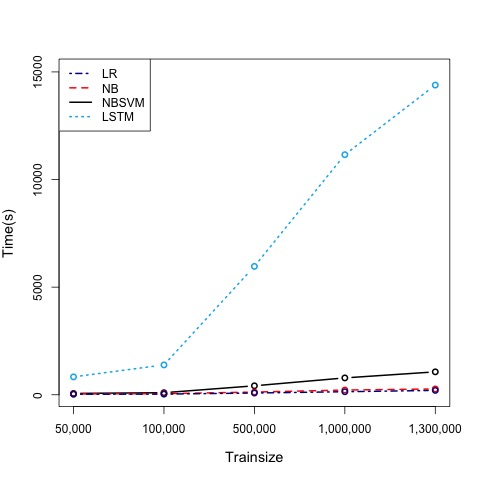
\includegraphics[width=\columnwidth]{../Plots/Compare_runtime.jpeg}
\captionof{figure}{Runtime of different methods in seconds}
\end{center}

\begin{center}
\centering
\label{fig:mse}
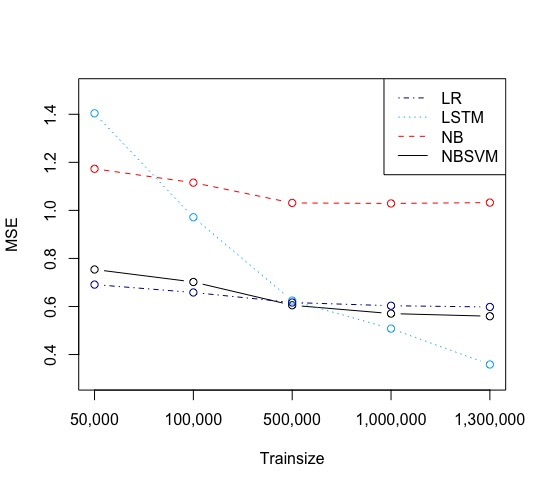
\includegraphics[width=\columnwidth]{../Plots/Compare_mse.jpeg}
\captionof{figure}{MSE of different methods}
\end{center}

% Tables need to be reshaped
\begin{table}
\centering
\caption{Runtime of different methods in seconds}
\label{table:runtime}
\begin{tabular}{l | lllll}
      & 50,000 & 100,000 & 500,000 & 1,000,000 & 1,300,000 \\ \hline
LR    & 25.84  & 30.49   & 80.85   & 141.24    & 203.03    \\
NB    & 39.62  & 50.66   & 125.71  & 219.25    & 269.72    \\
NBSVM & 62.34  & 95.78   & 416.81  & 783.34    & 1065.07   \\
LSTM  & 831.24 & 1386.66 & 5965.16 & 11154.41  & 14388.02 
\end{tabular}
\end{table}

\begin{table}]
\centering
\caption{MSE of different methods}
\label{table:mse}
\begin{tabular}{l | lllll}
      & 50,000 & 100,000 & 500,000 & 1,000,000 & 1,300,000 \\ \hline
LR    & 0.7067 & 0.6808  & 0.6433  & 0.6334    & 0.6310    \\
NB    & 1.1731 & 1.1154  & 1.0310  & 1.0288    & 1.0324    \\
NBSVM & 0.7540 & 0.7019  & 0.6050  & 0.5704    & 0.5594    \\
LSTM  & 1.4039 & 0.9714  & 0.6245  & 0.5078    & 0.3585   
\end{tabular}
\end{table}

% Subsection
\subsection{Memory Usage}


% Subsection
\subsection{Other Findings}
From Figure \ref{fig:mse_unclean} and Figure \ref{fig:runtime_unclean}, which show the different performance of NBSVM using the cleaned and uncleaned dataset as input, indicate that the usage of the cleaned dataset decreased the MSE but increased the speed of the model. A similar issue happened in NB. It could be argued that using a more complicated dataset which holds all information would yield better prediction results therefore no cleaning should be carried out before applying the models. However, the fact is the accuracy only increased for about 15\% in exchange of a decrease of 55\% of the speed (when the training size is 1,300,000). This implicates that cleaning the dataset denoised the data a lot yet retained most of the information and it suggests that it might be possible that the accuracy could be improved if we cleaned the dataset more carefully and still speeding up the whole process. 

\begin{center}
\centering
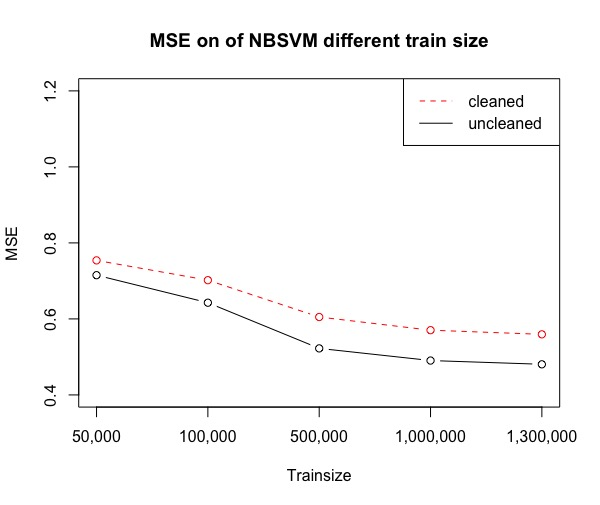
\includegraphics[width=\columnwidth]{../Plots/NBSVM_unclean_clean.jpeg}
\captionof{figure}{MSE of cleaned and uncleaned dataset}
\label{fig:mse_unclean}
\end{center}

\begin{center}
\centering
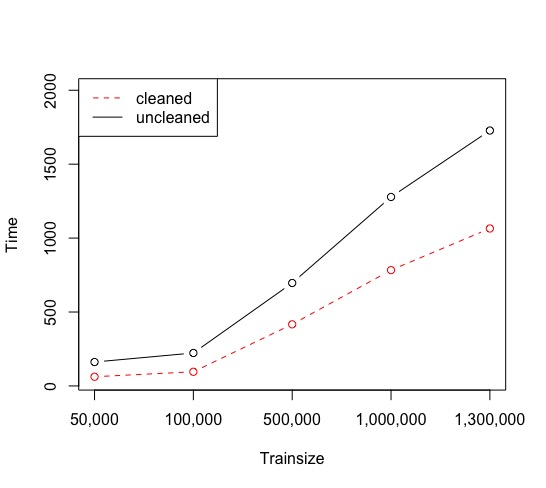
\includegraphics[width=\columnwidth]{../Plots/NBSVM_runtime_sample.jpeg}
\captionof{figure}{Runtime of cleaned and uncleaned dataset}
\label{fig:runtime_unclean}
\end{center}

\bibliography{bibfile}
\bibliographystyle{aaai}



\end{document}
